\documentclass{article}
\usepackage{amsmath}
\usepackage{graphicx}
\usepackage{siunitx}
\graphicspath{{./images/}}

\title{University Physics with Modern Physics Electromagnetism Notes}
\author{Chris Doble}
\date{December 2022}

% The Coulomb constant
\newcommand{\ke}{\frac{1}{4 \pi \epsilon_0}}

\begin{document}

\maketitle

\tableofcontents

\setcounter{section}{20}
\section{Electric Charge and Electric Field}

\subsection{Electric Charge}

\begin{itemize}
  \item Electrons have a much smaller mass than neutrons and protons

  \item Neutrons and protons have a very similar mass

  \item Electrons and protons have the same magnitude of charge

  \item The number of protons in an atom determins its \textbf{atomic number}

  \item If an electron is added to a neutral atom it becomes a \textbf{negative ion}, if one is removed it becomes a \textbf{positive ion} — this is called \textbf{ionisation}

  \item The \textbf{principle of conservation of charge} states that the algebraic sum of all the electric charges in any closed system is constant

  \item The electron or proton's magnitude of charge is a natural unit of charge — every observable amount of electric charge is an integer multiple of this
\end{itemize}

\subsection{Conductors, Insulators, and Incuded Charges}

\begin{itemize}
  \item \textbf{Conductors} pemit easy movement of charge, \textbf{insulators} do not

  \item Holding a charged object near an uncharged object causes free electrons in the latter to move away/towards the former, resulting in a net charge on either side — this is called \textbf{induced charge}
\end{itemize}

\subsection{Coulomb's Law}

\begin{itemize}
  \item The SI unit of charge is called one \textbf{coulomb} (1 C) and is defined such that $1.602176634\times10^{-19}$ C is equal to the charge of an electron or proton

  \item \textbf{Coulomb's law} describes the electric force between two point charges \[F = \frac{1}{4\pi\epsilon_0}\frac{|q_1q_2|}{r^2}\] where the \textbf{electric constant} $\epsilon_0 = 8.854 \times 10^{-12}\,\textrm{C}^2/\textrm{N}\cdot \textrm{m}^2$, $q_1$ and $q_2$ are the magnitudes of the charges, and $r$ is the distance between them

  \item The electric force is always directed along the line between the two charges, attracting opposite charges and repelling like charges

  \item $\frac{1}{4\pi\epsilon_0}$ can be approximated as $9.0 \times 10^9\,\textrm{N}\cdot\textrm{m}^2/\textrm{C}^2$

  \item The principle of superposition of forces also applies to electric charges
\end{itemize}

\subsection{Electric Field and Electric Forces}

\begin{itemize}
  \item The electric force on a charged object is exerted by the electric field created by other charged objects

  \item We can determine if there is an electric field at a point by placing a test charge $q_0$ there and seeing if it experiences an electric force — the electric field at that point (the electric force per unit charge) is then given by \[\mathbf{E} = \frac{\mathbf{F}}{q_0}\]

  \item Rearranging, the force experienced by a charge $q_0$ at a point is given by \[\mathbf{F} = q_0\mathbf{E}\]

  \item When considering an electric field produced by a point charge, the location of the point charge is called the \textbf{source point} and the location at which we're trying to determine the field is called the \textbf{field point}

  \item The electric field produced by a point charge is given by \[\mathbf{E} = \frac{1}{4\pi\epsilon_0} \frac{q}{r^2}\hat{\mathbf{r}}\] where $q$ is the charge of the point charge, $r$ is the distance between the source and field points, and $\hat{\mathbf{r}}$ is the unit vector from the source to the field point

  \item Unlike Coulomb's law this equation doesn't use the absolute value of $q$ meaning that the electric fields of positive charges point away from the charge, while those of negative charges point towards them

  \item In electrostatics, the electric field inside the material of a conductor (but not holes within the material) is $\mathbf{0}$
\end{itemize}

\subsection{Electric-Field Calculations}

\begin{itemize}
  \item The \textbf{principle of superposition of electric fields} states that the total electric field at a point $P$ is the vector sum of the fields at $P$ due to each point charge in the charge distribution \[\mathbf{E} = \mathbf{E}_1 + \mathbf{E}_2 + \cdots\]

  \item For a line charge distribution the \textbf{linear charge density} is represented by $\lambda$ (the charge per unit length, measured in $\textrm{C}/\textrm{m}$)

  \item For a surface charge distribution the \textbf{surface charge density} is represented by $\sigma$ (the charge per unit area, measured in $\textrm{C}/\textrm{m}^2$)

  \item For a volume charge distribution the \textbf{volume charge density} is represented by $\rho$ (the charge per unit volume, measured in $\textrm{C}/\textrm{m}^3$)

  \item The electric field of an infinitely long line charge along the $y$-axis is \[E = \frac{\lambda}{2\pi\epsilon_0 r}\]
\end{itemize}

\subsection{Electric Field Lines}

\begin{itemize}
  \item An \textbf{electric field line} is a line drawn through space such that its tangent at any point is in the direction of the electric field vector at  that point

  \item Fewer lines are drawn in areas where the electric field is weak and more lines are drawn in areas where it's strong
\end{itemize}

\subsection{Electric Dipoles}

\begin{itemize}
  \item An \textbf{electric dipole} is a pair of point charges of equal magnitude $q$ and opposite sign separated by a distance $d$

  \item The net force on an electric dipole in a uniform electric field is $\mathbf{0}$

  \item The \textbf{electric dipole moment} $\mathbf{p}$ of an electric dipole is a vector directed from the negative charge to the positive charge with magnitude $qd$

  \item The net torque on an electric dipole in a uniform electric field is $\mathbf{p} \times \mathbf{E}$ or $qEd\sin\phi$ where $\phi$ is the angle between the electric dipole and the electric field

  \item The potential energy of an electric dipole in a uniform electric field is \[U = -\mathbf{p} \cdot \mathbf{E}\]
\end{itemize}

\section{Gauss's Law}

\subsection{Calculating Electric Flux}

\begin{itemize}
  \item The electric flux of a uniform electric field through a flat surface $A$ is \[\Phi_E = \mathbf{E} \cdot \mathbf{A}\] where $\mathbf{A}$ is normal to $A$ and has a magnitude equal to its area

  \item The electric flux of a nonuniform electric field through a curved surface $A$ is \[\Phi_E = \int \mathbf{E} \cdot \mathbf{dA}\]
\end{itemize}

\subsection{Gauss's Law}

\begin{itemize}
  \item Gauss's law states that the total electric flux through a closed surface is equal to the total electric charge enclosed by the surface divided by $\epsilon_0$ \[\Phi_E = \oint \mathbf{E} \cdot \mathbf{dA} = \frac{Q_\textrm{enc}}{\epsilon_0}\]
\end{itemize}

\subsection{Applications of Gauss's Law}

\begin{itemize}
  \item Gauss's law can be used in two ways:

        \begin{itemize}
          \item If we know the charge distribution and it has enough symmetry to let us evaluate the integral in Gauss's law, we can find the field

          \item If we know the field, we can use Gauss's law to find the charge distribution
        \end{itemize}

  \item Under electrostatics, excess charge always lies of the surface of a conductor

  \item The electric field of an infinite line charge is \[\mathbf{E} = \ke \frac{2 \lambda}{r} \hat{\mathbf{r}}\]
\end{itemize}

\subsection{Charges on Conductors}

\begin{itemize}
  \item If there is excess charge at rest on a conductor, all of that charge must lie on the surface of the conductor and the electric field inside the conductor must be zero. If there is a cavity inside the conductor, the net charge on the cavity walls equals the amount of charge enclosed by the cavity

  \item Charges outside a conductor have no effect on the interior of the conductor, even if it has a cavity inside — this is why Faraday cages work

  \item At the surface of a conductor, the component of the electric field that is perpendicular to the surface is \[E_\perp = \frac{\sigma}{\epsilon_0}\]
\end{itemize}

\section{Electric Potential}

\subsection{Electric Potential Energy}

\begin{itemize}
  \item The electric potential energy of two point charges is \[U = \ke \frac{q_1 q_2}{r}\]

  \item The electric potential energy of a point charge $q_0$ and a collection of charges $q_1$, $q_2$, etc. is \[U = \frac{q_0}{4 \pi \epsilon_0} \left( \frac{q_1}{r_1} + \frac{q_2}{r_2} + \cdots \right) = \frac{q_0}{4 \pi \epsilon_0} \sum_i \frac{q_i}{r_i}\]

  \item For every electric field due to a static charge distribution, the force exterted by that field is conservative

  \item The total electric potential energy of a collection of charges $q_1$, $q_2$, etc. is \[U = \ke \sum_{i < j} \frac{q_i q_j}{r_{ij}}\] where $r_{ij}$ is the distance between $q_i$ and $q_j$
\end{itemize}

\subsection{Electric Potential}

\begin{itemize}
  \item \textbf{Potential} is potential energy per unit charge

  \item The unit of potential is the \textbf{volt}, equal to 1 joule per coulomb

  \item The potential difference between two points $V_{ab} = V_a - V_b$ is called the potential of $a$ with respect to $b$ and equals the amount of work done by the electric force when a unit ($\qty{1}{C}$) of charge moves from $a$ to $b$

  \item The electric potential due to a point charge is \[V = \ke \frac{q}{r}\]

  \item The electric potential due to a collection of point charges is \[V = \ke \sum_i \frac{q_i}{r_i}\]

  \item The electric potential due to a continuous charge distribution is \[V = \ke \int \frac{dq}{r}\]

  \item The electric potential difference between two points is given by \[V_a - V_b = \int_a^b \mathbf{E} \cdot d\mathbf{l} = \int_a^b E \cos \phi \,dl\]

  \item Positive charges tend to ``fall'' from high- to low-potential regions while negative charges do the opposite

  \item When a particle with charge $e = \qty{1.602e-19}{C}$ moves between two points with a potential difference of $\qty{1}{V} = \qty{1}{J/C}$ the change in energy is $U_a - U_b = qV_{ab} = (\qty{1.602e-19}{C})(\qty{1}{J/C}) = \qty{1.602e-19}{J}$ which is called 1 \textbf{electron volt}
\end{itemize}

\setcounter{subsection}{3}
\subsection{Equipotential Surfaces}

\begin{itemize}
  \item An \textbf{equipotential surface} is a three-dimensional surface on which the electric potential is the same at every point

  \item Because electric potential energy doesn't change as a test charge moves over an equipotential surface, the electric field can do no work and thus \textbf{field lines and equipotential surfaces are always perpendicular}

  \item When all charges are at rest, the surface of a conductor is an equipotential surface

  \item When all charges are at rest, the entire solid volume of a conductor is at the same potential
\end{itemize}

\subsection{Potential Gradient}

\begin{itemize}
  \item The relationship between $\mathbf{E}$ and $V$ is given by \[\mathbf{E} = -\nabla V = -\left( \frac{\partial V}{\partial x} \hat{\mathbf{i}} + \frac{\partial V}{\partial y} \hat{\mathbf{j}} + \frac{\partial V}{\partial z} \hat{\mathbf{k}} \right)\]

  \item If $E$ has a radial component $E_r$ with respect to an axis or a point and $r$ is the distance from that axis or point, then \[E_r = -\frac{\partial V}{\partial r}\]
\end{itemize}

\section{Capacitance and Dielectrics}

\subsection{Capacitors and Capacitance}

\begin{itemize}
  \item Any two conductors separated by an insulator (or a vacuum) form a \textbf{capacitor}

  \item The \textbf{capacitance} of a capacitor measures its ability to store charge \[C = \frac{Q}{V_{AB}}\]

  \item Capacitance is measured in \textbf{farads} where \[\qty{1}{F} = \qty{1}{C/V}\]

  \item The capacitance of a parallel plate capacitor in a vacuum is \[C = \epsilon_0 \frac{A}{d}\]
\end{itemize}

\subsection{Capacitors in Series and Parallel}

\begin{itemize}
  \item In a series connection, the magnitude of charge on all plates is the same

  \item The \textbf{equivalent capacitance} of a combination of capacitors is the capacitance of a single capacitor that would have equivalent behaviour

  \item In a series connection, the reciprocal of the equivalent capacitance equals the sum of the reciprocals of the individual capacitances \[\frac{1}{C_\textrm{eq}} = \frac{1}{C_1} + \frac{1}{C_2} + \cdots\] meaning the equivalent capacitance is always less than any individual capacitance

  \item In a parallel connection, the potential difference is the same for all capacitors

  \item In a parallel connection, the equivalent capacitance equals the sum of the individual capacitances \[C_\textrm{eq} = C_1 + C_2 + \cdots\] meaning the equivalent capacitance is always greater than any individual capacitance
\end{itemize}

\subsection{Energy Storage in Capacitors and Electric-Field Energy}

\begin{itemize}
  \item The potential energy stored in a capacitor is \[U = \frac{Q^2}{2 C} = \frac{1}{2} C V^2 = \frac{1}{2} Q V\]

  \item The \textbf{energy density} of a parallel plate capacitor is its energy per unit volume \[u = \frac{\frac{1}{2} C V^2}{A d} = \frac{1}{2} \epsilon_0 E^2\]
\end{itemize}

\subsection{Dielectrics}

\begin{itemize}
  \item \textbf{Dielectrics} are nonconducting materials

  \item Most capacitors have a dielectric material between their plates because

        \begin{enumerate}
          \item It preserves the distance between the plates

          \item It increases the maximum potential difference between the plates by avoiding \textbf{dielectric breakdown} when the material between the plates becomes ionized and becomes conductive — this happens more easily for air

          \item It increases the capacitance by decreasing the potential difference for a given charge
        \end{enumerate}

  \item The \textbf{dielectric constant} of a material is defined as \[K = \frac{C}{C_0}\] where $C_0$ is the capacitance of a capacitor with vacuum between the plates and $C$ is the capacitance of the same capacitor with the material between the plates

  \item If $E_0$ is the magnitude of the electric field between the plates of a parallel plate capacitor when separated by a vacuum and $E$ is the magnitude when separated by a dielectric then \[E = \frac{E_0}{K}\]

  \item The electric field (and electric potential) are reduced because the dielectric becomes \textbf{polarized} and an induced surface charge appears of magnitude \[\sigma_i = \sigma \left( 1 - \frac{1}{K} \right)\]

  \item The \textbf{permittivity} of a dielectric is defined as \[\epsilon = K \epsilon_0\]

  \item The capacitance of a parallel plate capacitor with dielectric between the plates is thus \[C = K C_0 = K \epsilon_0 \frac{A}{d} = \epsilon \frac{A}{d}\] and the electric energy density is \[u = \frac{1}{2} K \epsilon_0 E^2 = \frac{1}{2} \epsilon E^2\]

  \item The maximum electric-field magnitude that a material can withstand without the occurence of breakdown is called its \textbf{dielectric strength} and is denoted $E_m$
\end{itemize}

\subsection{Molecular Model of Induced Charge}

\begin{itemize}
  \item If a material is comprised of polar molecules where the net charge of the molecule is $0$ but the charge isn't distributed equally, electric fields cause the molecules to rotate which induces a charge

  \item Even if a material isn't comprised of polar molecules, electric fields cause molecules' positive and negative charges to separate slightly resulting in a dipole which again experiences a torque

  \item The charges in conductors are free to move so they're known as \textbf{free charges} while the charges in dielectrics aren't so they're known as \textbf{bound charges}
\end{itemize}

\subsection{Gauss's Law in Dielectrics}

\begin{itemize}
  \item Gauss's Law in a dielectric material relates the flux of $K \mathbf{E}$ through the surface to the amount of free (not bound) charge enclosed by the surface \[\oint K \mathbf{E} \cdot d\mathbf{A} = \frac{Q_\textrm{encl-free}}{\epsilon_0}\]

  \item This shows that filling a volume with a dielectric with relative permittivity $K$ reduces the magnitude of the electric field by a factor of $1 / K$
\end{itemize}

\section{Current, Resistance, and Electromotive \\ Force}

\subsection{Current}

\begin{itemize}
  \item A \textbf{current} is any motion of charge from one region to another

  \item The \textbf{drift velocity} $\mathbf{v_d}$ of a current is the velocity of its particles

  \item While a current may come about through the movement of negative and/or positive charges, \textbf{conventional current} dictates that by convention we describe currents as if they were carried by positive charges

  \item The unit of current is the \textbf{ampere} which is defined to be one coulomb per second \[\qty{1}{A} = \qty{1}{C/s}\]

  \item The \textbf{charge concentration} $n$ is the number of moving charged particles per unit volume

  \item The current through an area is given by \[I = \frac{dQ}{dt} = n |q| v_d A\]

  \item The \textbf{current density} is the current per unit cross-sectional area \[\mathbf{J} = n q \mathbf{v_d}\]
\end{itemize}

\subsection{Resistivity}

\begin{itemize}
  \item The \textbf{resistivity} $\rho$ of a material is defined by \textbf{Ohm's law} \[\rho = \frac{E}{J}\]

  \item The unit of resistivity is ohm-meters ($\unit{\Omega m}$)

  \item The reciprocal of resistivity is \textbf{conductivity}

  \item Materials that obey Ohm's law are called \textbf{ohmic} or \textbf{linear} conductors

  \item Materials that don't obey Ohm's law are called \textbf{nonohmic} or \textbf{nonlinear} conductors

  \item The resistivity of a metallic conductor nearly always increases with increasing temperature \[\rho(T) = \rho_0 [1 + \alpha (T - T_0)]\] where $\rho_0$ is the resistivity at reference temperature $T_0$ and $\alpha$ is the \textbf{temperature coefficient of resistivity}

  \item The resistivity of semiconductors decreases with increasing temperature

  \item Some materials exhibit \textbf{superconductivity} where their resistivity drops to 0 below a critical temperature
\end{itemize}

\subsection{Resistance}

\begin{itemize}
  \item The ratio of the voltage and current in a conductor is called its \textbf{resistance} \[R = \frac{V}{I} = \frac{\rho L}{A}\] where $\rho$ is the resistivity of the conductor, $L$ is its length, and $A$ is its cross-sectional area

  \item If $\rho$ is constant (as in ohmic materials), then $R$ is also constant

  \item The unit of resistance is the ohm \[\qty{1}{\Omega} = \qty{1}{V/A}\]

  \item Because the resistivity of a material varies with temperature, so too does the resistance of a specific conductor \[R(T) = R_0 [1 + \alpha (T - T_0)]\]

  \item A device made to have a specific resistance is called a \textbf{resistor}
\end{itemize}

\subsection{Electromotive Force and Circuits}

\begin{itemize}
  \item When a charge goes around a complete circuit and returns to its starting position its electric potential energy must be the same, but it experienced losses due to resistance along the way

  \item \textbf{Electromotive force} or \textbf{emf} $\mathcal{E}$ is the influence that makes current flow from lower to higher potential in a circuit and restores its original potential energy

  \item A device that provides emf is called a \textbf{source of emf}

  \item The SI unit of emf is the volt

  \item In an \textbf{ideal source of emf}

        \begin{itemize}
          \item The potential difference between its terminals is constant regardless of the current passing through it

          \item $\mathcal{E} = V = I R$
        \end{itemize}

  \item Real sources of emf have \textbf{internal resistance} $r$ that reduce the \textbf{terminal voltage} \[V_{ab} = \mathcal{E} - I r\]

  \item Real sources of emf can be modelled as an ideal source of emf $\mathcal{E}$ in series with a resistor $r$
\end{itemize}

\subsection{Energy and Power in Electric Circuits}

\begin{itemize}
  \item \textbf{Power} is the time rate change of energy transfer \[P = V I\] where $V$ is the voltage across a circuit element and $I$ is the current in it

  \item The SI unit of power is the watt \[\qty{1}{W} = \qty{1}{J/s}\]

  \item If the circuit element is a resistor then $V = IR$ and \[P = V I = I^2 R = \frac{V^2}{R}\]

  \item If the circuit element is a source of emf outputting power then \[P = V I = (\mathcal{E} - I r) I = \mathcal{E} I - I^2 r\] where the $\mathcal{E} I$ term is the power generated by the element and the $I^2 r$ term is the power dissipated by its internal resistance

  \item If the circuit element is a source of emf consuming power (charging) then \[P = V I = (\mathcal{E} + I r) I = \mathcal{E} I + I^2 r\] where the terms are the same as above
\end{itemize}

\subsection{Theory of Metallic Conduction}

\begin{itemize}
  \item The average time between collisions of an electron and positive ions is called the \textbf{mean free time} $\tau$

  \item The resistivity of a metal can be approximated as \[\rho = \frac{m}{n e^2 \tau}\] where $m$ is the mass of an electron, $n$ is the number of free electrons per unit volume, $e$ is the charge of an electron, and $\tau$ is the mean free time
\end{itemize}

\section{Direct-Current Circuits}

\subsection{Resistors in Series and Parallel}

\begin{itemize}
  \item Circuit elements connected one after another with a single current path between them are said to be connected in \textbf{series}

  \item The current is the same for all circuit elements connected in series

  \item Circuit elements connected such there is an alternate current path for each element are said to be connected in \textbf{parallel}

  \item The potential difference / voltage is the same for all circuit elements connected in parallel

  \item For any combination of resistors we can always find a single resistor that could replace the combination and result in the same current and potential difference — the resistance of this resistor is called the \textbf{equivalent resistance}

  \item The equivalent resistance of a series combination of resistors equals the sum of the individual resistances \[R_\textrm{eq} = R_1 + R_2 + \cdots\]

  \item The reciprocal of the equivalent resistance of a parallel combination of resistors equals the sum of the reciprocals of the individual resistances \[\frac{1}{R_\textrm{eq}} = \frac{1}{R_1} + \frac{1}{R_2} + \cdots\]
\end{itemize}

\subsection{Kirchhoff's Rules}

\begin{itemize}
  \item A \textbf{junction} in a circuit is a point where three or more conductors meet

  \item A \textbf{loop} is any closed conducting path

  \item \textbf{Kirchhoff's junction rule} states that the sum of the currents into any junction equals zero \[\sum I = 0\]

  \item \textbf{Kirchhoff's loop rule} states that the sum of the potential differences around any loop equals zero \[\sum V = 0\]

  \item Kirchhoff's rules can be used to analyse circuits by following these steps \\ 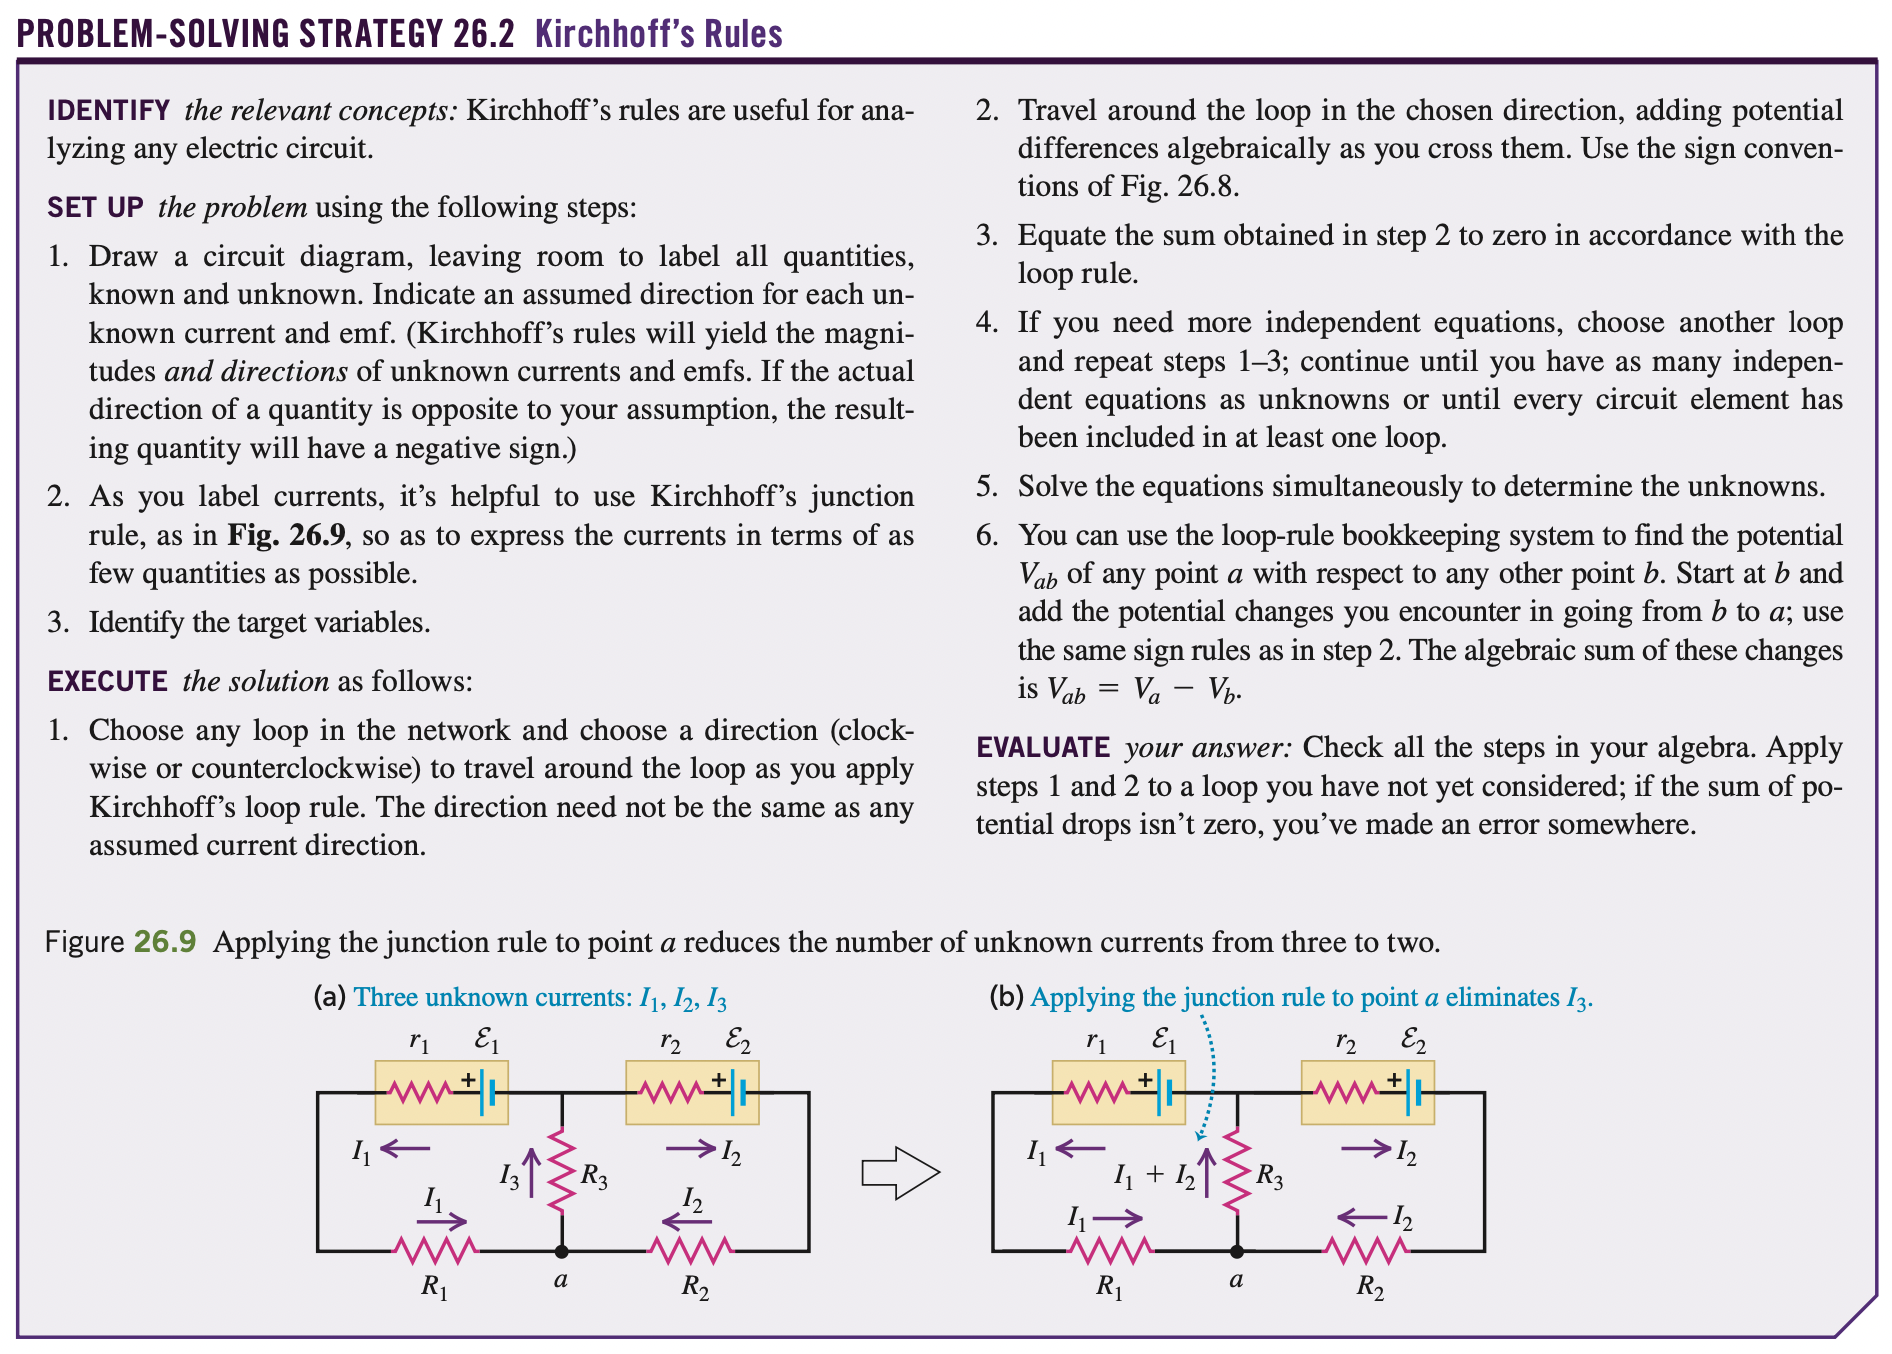
\includegraphics[scale=0.337]{kirchhoffs-rules}
\end{itemize}

\end{document}